\documentclass[tikz,11pt]{standalone}
\usepackage{newtxtext,newtxmath}
\usepackage{xcolor}

% Define sizes in cm
\def\totalwidth{15.92}
\def\totalheight{6.5}
\def\widthA{7.95}
\def\widthB{7.5}

\tikzstyle{dot}                  = [fill=black,anchor=center,minimum width=1cm]
\tikzstyle{incoherent tunneling} = [->,>=latex,ultra thick,blue!80,shorten <=1pt,shorten >=1pt]
\tikzstyle{coherent tunneling}   = [->,>=stealth,thick,densely dashed,shorten <=1pt,shorten >=1pt,red!60]
\tikzstyle{ket}                  = [left,inner sep=1pt]

\begin{document}
    \usetikzlibrary{calc,positioning}

    \begin{tikzpicture}
        \useasboundingbox[] (0,0) grid (\totalwidth,-\totalheight);
        
        % Part (a)
        \begin{scope}[local bounding box=A]
            \useasboundingbox (0,0) rectangle (\widthA, -\totalheight);

	      % Letter
            \node[anchor=north west, inner sep=3pt] at (current bounding box.north west) {\small (a)} ;

            \begin{scope}[shift={(A.center)}, inner sep=0pt]
                \node (c) at (-0.1,0) [minimum width=3.cm,minimum height=4.5cm] {};

                \node[dot]  (1) at (c.north west) {};
                \node[dot]  (2) at (c.north) {};
                \node[dot]  (3) at (c.north east) {};
                \node[dot]  (4) at ($(c.west)!0.5!(c.north west)$) {};
                \node[dot]  (5) at ($(c.east)!0.5!(c.north east)$) {};
                \node[dot]  (6) at (c.west) {};
                \node[dot]  (7) at (c.center) {};
                \node[dot]  (8) at (c.east) {};
                \node[dot]  (9) at ($(c.center)!0.5!(c.south)$) {};
                \node[dot] (10) at (c.south west) {};
                \node[dot] (11) at (c.south) {};
                \node[dot] (12) at (c.south east) {};

                \node[above=1ex] at (2) {\small $\textcolor{red!60}{\frac{g}{2}\sin \bar{\theta}}$};

                {\scriptsize
                \node[ket,anchor=east]            at  (1.west)  {$\left|+,\!n_{L},\!n_{R}\right\rangle$};
                \node[ket,anchor=north,below=1ex] at  (2.south) {$\left|-,\!n_{L}\!\!+\!\!1,\!n_{R}\right\rangle$};
                \node[ket,anchor=west]            at  (3.east)  {$\left|+,\!n_{L}\!\!+\!\!1,\!n_{R}\!\!-\!\!1\right\rangle$};
                \node[ket,anchor=east]            at  (4.west)  {$\left|\alpha \sigma,\!n_{L},\!n_{R}\right\rangle$};
                \node[ket,anchor=west]            at  (5.east)  {$\left|\alpha \sigma,\!n_{L}\!\!+\!\!1,\!n_{R}\!\!-\!\!1\right\rangle$};
                \node[ket,anchor=east]            at  (6.west)  {$\left|-,\!n_{L},\!n_{R}\right\rangle$};
                \node[ket,anchor=south,above=1ex] at  (7.north) {$\left|+,\!n_{L},\!n_{R}\!\!-\!\!1\right\rangle$};
                \node[ket,anchor=west]            at  (8.east)  {$\left|-,\!n_{L}\!\!+\!\!1,\!n_{R}\!\!-\!\!1\right\rangle$};
                \node[ket,anchor=west]            at  (9.east)  {$\left|\alpha \sigma,\!n_{L},\!n_{R}\!\!-\!\!1\right\rangle$};
                \node[ket,anchor=east]            at (10.west)  {$\left|+,\!\textcolor{blue}{n_{L}\!\!-\!\!1,\!n_{R}\!\!-\!\!1}\right\rangle$};
                \node[ket,anchor=north,below=1ex] at (11.south) {$\left|-,\!\textcolor{blue}{n_{L},\!n_{R}\!\!-\!\!1}\right\rangle$};
                \node[ket,anchor=west]            at (12.east)  {$\left|+,\!\textcolor{blue}{n_{L},\!n_{R}\!\!-\!\!2}\right\rangle$};
                }
                
                \draw[coherent tunneling]  (1.east) to[bend left=40]  (2.west) edge[bend left=40] (1.east);
                \draw[coherent tunneling]  (2.east) to[bend left=40]  (3.west) edge[bend left=40] (2.east);
                \draw[coherent tunneling]  (6.east) to[bend left=40]  (7.west) edge[bend left=40] (6.east);
                \draw[coherent tunneling]  (7.east) to[bend left=40]  (8.west) edge[bend left=40] (7.east);
                \draw[coherent tunneling] (10.east) to[bend left=40] (11.west) edge[bend left=40] (10.east);
                \draw[coherent tunneling] (11.east) to[bend left=40] (12.west) edge[bend left=40] (11.east);

                \draw[incoherent tunneling] 
                    ([xshift=-3pt]1.center) -- ([xshift=-3pt]4.center);
                \draw[incoherent tunneling,thick,densely dashed,blue!60!black!30]     
                    ([xshift=3pt]4.center) -- ([xshift=3pt]1.center);

                \draw[incoherent tunneling] 
                    ([xshift=-3pt]3.center) -- ([xshift=-3pt]5.center);
                \draw[incoherent tunneling,thick,densely dashed,blue!60!black!30]
                    ([xshift=3pt]5.center) -- ([xshift=3pt]3.center);

                \draw[incoherent tunneling] 
                    ([xshift=-3pt]4.center) -- ([xshift=-3pt]6.center);
                \draw[incoherent tunneling,thick,densely dashed,blue!60!black!30]
                    ([xshift=3pt]6.center) -- ([xshift=3pt]4.center);

                \draw[incoherent tunneling] 
                    ([xshift=-3pt]5.center) -- ([xshift=-3pt]8.center);
                \draw[incoherent tunneling,thick,densely dashed,blue!60!black!30]
                    ([xshift=3pt]8.center) -- ([xshift=3pt]5.center);

                \draw[incoherent tunneling] 
                    ([xshift=-3pt]7.center) -- ([xshift=-3pt]9.center);
                \draw[incoherent tunneling,thick,densely dashed,blue!60!black!30]
                    ([xshift=3pt]9.center) -- ([xshift=3pt]7.center);

                \draw[incoherent tunneling] 
                    ([xshift=-3pt]9.center) -- ([xshift=-3pt]11.center);
                \draw[incoherent tunneling,thick,densely dashed,blue!60!black!30]
                    ([xshift=3pt]11.center) -- ([xshift=3pt]9.center);

                \draw[<->, >=latex,thick,densely dotted,gray] (6) -- (10) node[midway,left=0.5ex] {\small $\bar{\delta}\approx \omega$};
            \end{scope}
        \end{scope}

        % Part (b)
        \begin{scope}[shift={(A.north east)}, local bounding box=B, inner sep=0pt]
            \useasboundingbox[] (0,0) grid (\widthB, -\totalheight);

            % Include plot
            \node[anchor=north east,inner sep=0pt,outer sep=0pt] at (current bounding box.north east) {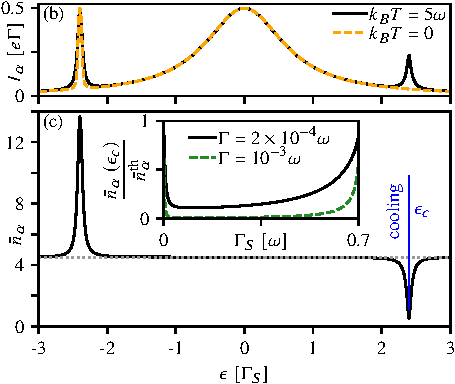
\includegraphics{cps-local-cooling-plot.pdf}};
        \end{scope}
    \end{tikzpicture}
\end{document}

